
\graphicspath{{../suyluancungbi/sumi/}}
\begingroup
\AddToShipoutPicture*{\put(115,595){
\includegraphics[scale=0.85]{sumi}}} % %Image background
%\AddToShipoutPicture*{\put(20,60){
\includegraphics[scale=0.75]{shape1}}} % %Image background
%\AddToShipoutPicture*{\put(70,260){
\includegraphics[scale=0.75]{cd1}}} % %Image background
\AddToShipoutPicture*{\put(48,255){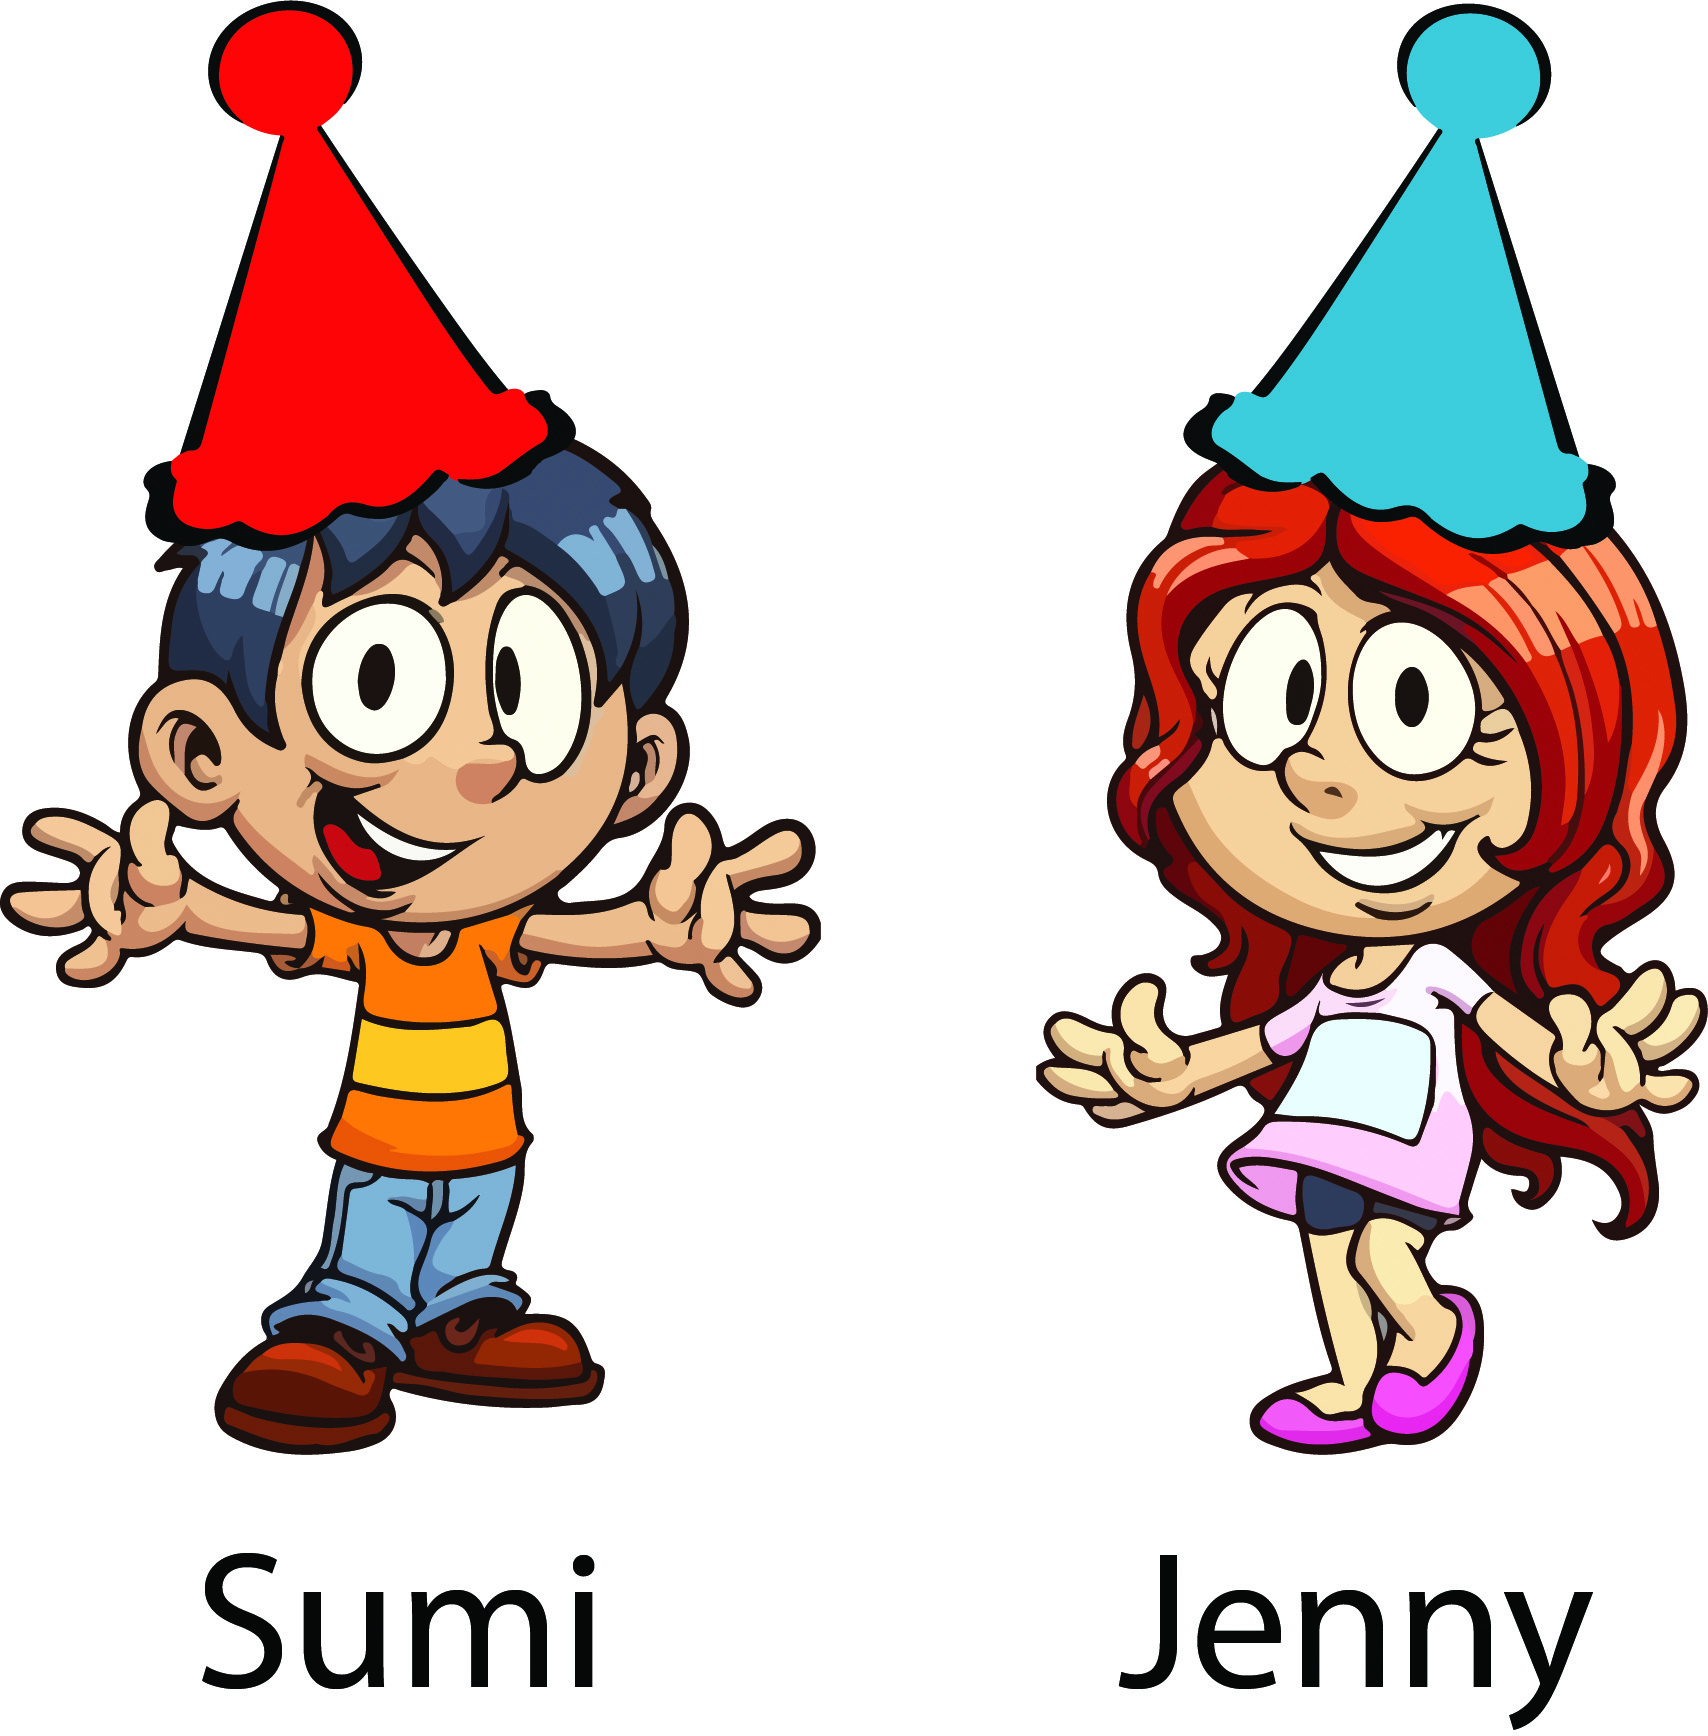
\includegraphics[scale=0.3]{h1}}} % %Image background
\centering
\endgroup
\vspace*{35pt}

	\textbf{\color{toancuabi}\textit{Sumi và Jenny là một đôi bạn rất  thân và đặc biệt là cả hai bạn đều rất thích học  Toán. Chú Jason, bố của Jenny là một thầy giáo dạy Toán nên có rất nhiều các câu đố vui hóc búa để thử thách các  bạn nhỏ. 
	\vskip 0.2cm
	Hôm nay Sumi sang chơi nhà Jenny. Như thường lệ, điều Sumi chờ đợi nhất chính là những câu đố của chú Jason.
	\vskip 0.2cm
	Không để các bạn phải đợi lâu, chú Jason lấy ra một chiếc mũ màu đỏ, một chiếc mũ màu xanh, và bắt đầu chuỗi câu đố của mình.}}
	
	\vskip 0.1cm
	\vspace*{1pt}
	\textbf{\color{toancuabi}Câu đố $\pmb1$}	


\vspace*{-20pt}\begin{adjustwidth}{130pt}{0pt}
	-- Hai con hãy nhắm mắt lại một lúc, để ta có thể đội cho mỗi người một chiếc mũ nhé! -- Chú Jason nói
	-- Được rồi, các con có thể mở mắt ra. Sumi, con có biết mũ của mình màu gì không?
	\vskip 0.1cm
	Sumi nhìn Jenny và trả lời ngay lập tức:
	\vskip 0.1cm
	-- Màu đỏ ạ.
	\vskip 0.1cm
	-- Tại sao con lại biết mũ của mình màu đỏ? -- Chú Jason hỏi tiếp.
	\vskip 0.1cm
	-- Con thấy Jenny đội mũ màu xanh, nên chiếc mũ của con phải là màu đỏ ạ. -- Sumi trả lời.
\end{adjustwidth}
%\begingroup
%\AddToShipoutPicture*{\put(0,295){
\includegraphics[scale=1]{shape2.pdf}}} % %Image background
%\AddToShipoutPicture*{\put(80,545){
\includegraphics[scale=0.75]{cd2.pdf}}} % %Image background
%\AddToShipoutPicture*{\put(240,-10){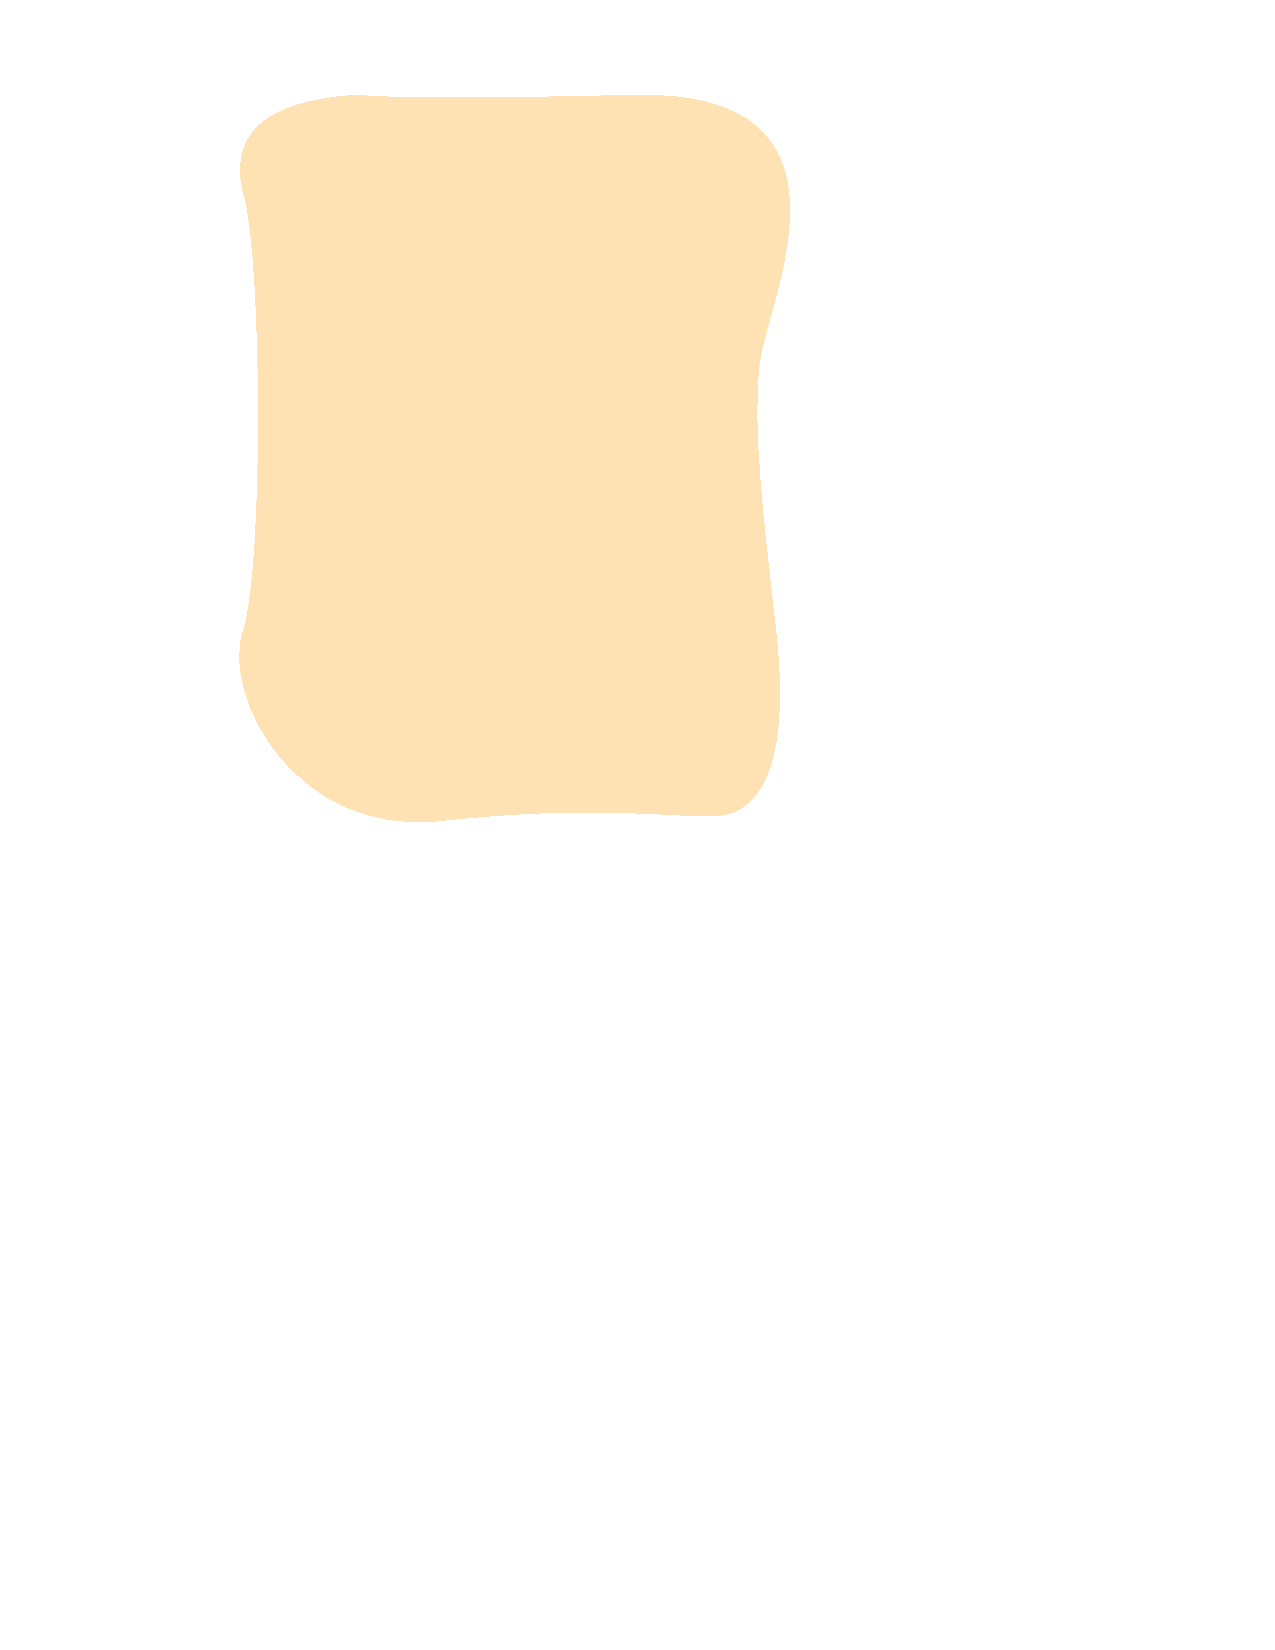
\includegraphics[scale=0.75]{shape3.pdf}}} % %Image background
%\AddToShipoutPicture*{\put(350,725){
\includegraphics[scale=0.75]{cd3.pdf}}} % %Image background
%\AddToShipoutPicture*{\put(70,330){
\includegraphics[scale=0.25]{sumi/h2}}} % %Image background
%\AddToShipoutPicture*{\put(340,365){\includegraphics[scale=0.25]{sumi/h3}}} % %Image background
%\AddToShipoutPicture*{\put(70,25){\includegraphics[scale=0.25]{sumi/h5}}} % %Image background
%\AddToShipoutPicture*{\put(340,20){\includegraphics[scale=0.25]{sumi/h4}}} % %Image background
%\AddToShipoutPicture*{\put(110,275){
\includegraphics[scale=0.75]{cd5.pdf}}}
%\AddToShipoutPicture*{\put(350,325){
\includegraphics[scale=0.75]{cd4.pdf}}} % %Image background
%\centering
%\endgroup
%\begin{adjustwidth}{0pt}{80pt}
	\textbf{\color{toancuabi}Câu đố $\pmb2$}
	\vskip 0.1cm
	Chú Jason lấy thêm một chiếc mũ màu đỏ. Chú lại yêu cầu hai bạn nhắm mắt lại, và đội cho mỗi bạn một chiếc mũ. Sau đó, chú giấu chiếc mũ còn lại đi.
	\vskip 0.1cm
	-- Bây giờ, các con mở mắt ra nào. Sumi, con có biết mũ của mình màu gì không? -- Chú  Jason hỏi.
	\vskip 0.1cm
	-- Dạ không ạ. -- Sumi nhìn Jenny, nhưng lần này cậu không đoán được màu mũ của mình.
	\vskip 0.1cm
	\begin{multicols}{2}
		\begin{figure}[H]
			\centering
			\vspace*{-5pt}
			\captionsetup{labelformat= empty, justification=centering}
			
\includegraphics[width=0.95\linewidth]{h2}
			\vspace*{-20pt}
		\end{figure}
		-- Còn Jenny, con có biết mình đội mũ màu  gì không?
		\vskip 0.1cm
		-- Màu đỏ ạ. -- Jenny trả lời ngay lập tức.
		\vskip 0.1cm
		-- Con hãy giải thích cho bố xem tại sao nào?
		\vskip 0.1cm
		-- Nếu con đội mũ màu xanh thì chỉ còn lại hai chiếc mũ màu đỏ, và khi đó Sumi sẽ biết ngay là bạn ý đội chiếc mũ màu đỏ ạ. Do Sumi không đoán được bạn ý đội mũ màu gì, nên chiếc mũ của con phải là màu đỏ ạ. – Jenny giải thích.
		%	\end{adjustwidth}
	\end{multicols}
	\begin{multicols}{2}
		\textbf{\color{toancuabi}Câu đố $\pmb3$}
		\vskip 0.1cm
		Đúng lúc này thì bé Julia đi học về, và đòi chơi cùng anh Sumi và chị Jenny. Chú Jason yêu cầu ba bạn nhỏ nhắm mắt lại và dùng hai chiếc mũ đỏ, một chiếc mũ xanh để đội cho mỗi bạn một chiếc mũ.
		\vskip 0.1cm
		-- Các con mở mắt ra nào. Sumi, con có biết mũ của mình màu gì không?
		\vskip 0.1cm
		-- Màu xanh ạ! -- Sumi trả lời rất nhanh.
		\vskip 0.1cm
		-- Con cũng đội mũ màu xanh ạ! -- Julia  nhanh nhẩu.
		\vskip 0.1cm
		-- Màu xanh? Con có chắc không, Julia? -- Chú Jason hỏi lại.
		\vskip 0.1cm
		-- Ah, con bị nhầm rồi ạ. Bố dùng hai chiếc mũ đỏ, một chiếc mũ xanh. Anh Sumi đội mũ xanh, chị Jenny đội mũ đỏ, như vậy con sẽ đội mũ đỏ ạ. – Julia sửa lại.
		\begin{figure}[H]
			\centering
			\vspace*{-5pt}
			\captionsetup{labelformat= empty, justification=centering}
			\includegraphics[width=1\linewidth]{h3}
			\vspace*{-10pt}
		\end{figure}
	\end{multicols}
	
	
	\textbf{\color{toancuabi}Câu đố $\pmb4$}
	\vskip 0.1cm
	-- Tốt lắm! Bây giờ sẽ là một thử thách khó hơn cho các con. -- Chú Jason nói; rồi chú lấy thêm một chiếc mũ đỏ và một chiếc mũ xanh. Như vậy, có tổng cộng ba chiếc mũ đỏ và hai chiếc mũ xanh trên bàn. Chú lại yêu cầu cả ba bạn nhắm mắt lại, rồi đội cho mỗi bạn một chiếc mũ. Sau đó, chú giấu hai chiếc mũ còn lại đi.
	\vskip 0.1cm
	-- Jenny, con có biết mình đội mũ màu gì không?
	\vskip 0.1cm
	-- Con đội mũ đỏ ạ. -- Jenny trả lời.
	\vskip 0.1cm
	-- Vậy thì con đội mũ màu xanh rồi. -- Sumi  nói tiếp.
	\vskip 0.1cm
	Theo các bạn, Sumi nói có đúng không? Vì sao?
	\begin{figure}[H]
		\centering
		\vspace*{-5pt}
		\captionsetup{labelformat= empty, justification=centering}
		\includegraphics[width=0.55\textwidth]{h5}
		\vspace*{-10pt}
	\end{figure}
	
	\textbf{\color{toancuabi}Câu đố $\pmb5$}
	\vskip 0.1cm
	Các bạn nhỏ đòi chú Jason đố thêm một lần nữa. Chú vẫn dùng ba chiếc mũ đỏ và hai chiếc mũ xanh để đội cho mỗi bạn một chiếc.
	\vskip 0.1cm
	-- Sumi, con có biết mình đội mũ màu gì không?
	\vskip 0.1cm
	-- Còn Jenny, con đội mũ màu gì?
	\vskip 0.1cm
	-- Con cũng không biết ạ. -- Jenny lắc đầu.
	\vskip 0.1cm
	-- Vậy thì Julia, con đội mũ màu gì?
	\vskip 0.1cm
	Các bạn hãy giúp Julia trả lời câu hỏi nhé!
	\begin{figure}[H]
		\centering
		\vspace*{-5pt}
		\captionsetup{labelformat= empty, justification=centering}
		\includegraphics[width=0.5\textwidth]{h4}
		\vspace*{-10pt}
	\end{figure}